% !TEX root = ../../prj4projektdokumentation.tex

\chapter{Kommunikationsprotokoller}
\label{ch:KomProtokol}

\section{TCP protokol}
\label{sec:TCPprotokol}
Mellem kommunikationsmodulet og kontrolmodulet er anvendt en TCP protokol. TCP er valgt, da systemet ikke kræver hurtig, men derimod en meget pålidelig datatransmission. PLC'en anvender stikstandarden RJ-45 og har mulighed for at kommunikere med hastighederne 10/100 Mb/s. Her anvendes .....
PLC'en er opsat som client, der forespørger data fra Arduinoen, som svarer med det forespurgte data. Kommunikation over TCP forbindelsen anvender protokollen vist på figur \ref{fig:TCPprotokol}.

\begin{figure}[H] % (alternativt [H])
	\centering
	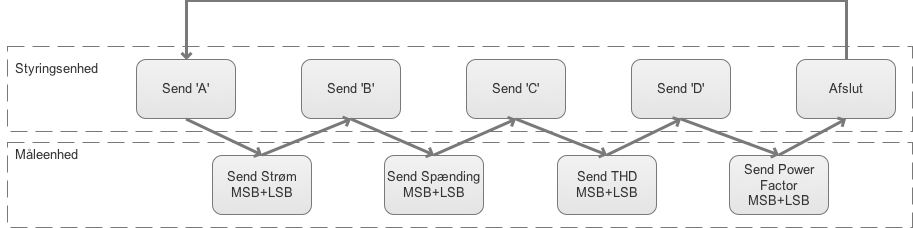
\includegraphics[width=\textwidth]{Figure/UARTprotokol}
	\caption{Protokol for kommunikation mellem kommunikationsmodul og kontrolmodul}
	\label{fig:TCPprotokol}
\end{figure}

\section{UART protokol}
\label{sec:UARTprotokol}
UART protokollen anvendes mellem Måleenheden og Styringsenheden. Opsætning af UART forbindelse overholder indstillingerne i Tabel \ref{tab:UARTprotokol}. Data som transmitteres over UART forbindelsen sendes i pakker af 8-bit. Da værdier for strøm, spænding, power factor og THD er uint16 værdier, skal der for hver værdi sendes to pakker, henholdsvis MSB og LSB. 

Kommunikation over UART forbindelsen skal overholde følgende protokol, se Figur \ref{fig:UARTprotokol}.
\begin{figure}[H] % (alternativt [H])
	\centering
	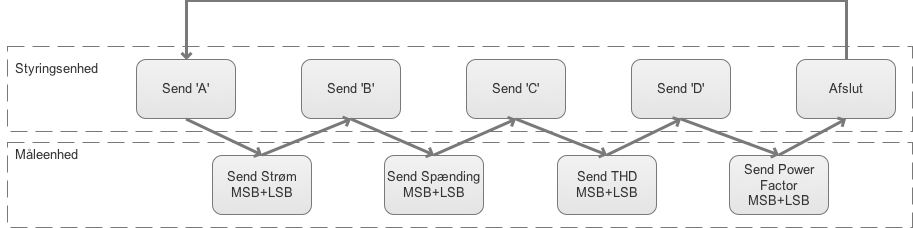
\includegraphics[width=\textwidth]{Figure/UARTprotokol}
	\caption{Protokol for kommunikation mellem Måleenhed og Styringsenhed}
	\label{fig:UARTprotokol}
\end{figure}

\begin{table}[h]
	\centering
	\caption{UART protokol}
	\label{tab:UARTprotokol}
	\begin{tabular}{@{}lll@{}}
		\toprule
							& Indstilling       		& Bemærkning \\ \midrule
		Mode       		& Full UART (Rx+Tx) &            \\
		BaudRate 	  & 9600             		 &            \\
		DataBits    	& 8             			    &            \\
		ParityType 	  	& None     			         &            \\
		Stopbits    	& 1               				  &            \\
		Flowcontrol 	& None         		     &           \\ \hline
	\end{tabular}
\end{table}
